\documentclass[aspectratio=169,10pt]{beamer}
\usepackage{graphicx}
\usepackage{booktabs}
\usepackage{listings}
\usepackage{xcolor}
\usepackage{hyperref}
\usepackage{tikz}
\usetheme{Madrid}
\usecolortheme{seahorse}

% 设置中文字体 - XeLaTeX 下使用系统字体
\usepackage[UTF8, heading=true]{ctex}
\setCJKsansfont[BoldFont={Heiti SC}, ItalicFont={Heiti SC}]{Heiti SC}
\setCJKmainfont{Songti SC}

% 代码样式
\lstset{
    language=C++,
    basicstyle=\tiny\ttfamily,
    keywordstyle=\color{blue}\bfseries,
    stringstyle=\color{red},
    commentstyle=\color{green!60!black},
    numbers=left,
    numberstyle=\tiny\color{gray},
    breaklines=true,
    showstringspaces=false
}

% 标题信息
\title{Shell-Derived Resident Partition Model}
\subtitle{MPI通信优化的新访问模型}
\author{汇报人}
\institute{}
\date{\today}

% 颜色定义
\definecolor{primary}{RGB}{30, 58, 95}
\definecolor{secondary}{RGB}{135, 206, 235}
\definecolor{accent}{RGB}{255, 107, 107}
\definecolor{success}{RGB}{144, 238, 144}
\definecolor{warning}{RGB}{255, 215, 0}

\begin{document}

% ============ 第1页: 标题页 ============
\begin{frame}
\titlepage
\end{frame}

% ============ 第2页: 目录 ============
\begin{frame}{目录}
\tableofcontents
\end{frame}

% ============ 第3页: 问题背景 ============
\section{问题背景}
\begin{frame}{现有方案的瓶颈}
\begin{block}{当前 Legacy AccessPattern 方案}
\begin{itemize}
    \item 每个 \texttt{<->} 表达式独立执行完整的 root-centric 通信周期
    \item 约 \textbf{10+ 次 MPI 调用} / 表达式
    \item 中间张量经历不必要的 Gather/Scatter 往返
    \item View1D 间接寻址带来额外开销
    \item 每 \texttt{<->} 独立初始化 AccessPattern、PackPlan、SYCL buffer
\end{itemize}
\end{block}

\bigskip
\begin{alertblock}{性能差距}
\begin{tabular}{lcc}
    \toprule
    用例 & 效率比 & 核心原因 \\
    \midrule
    imageAdjustment1.0 & ~20x & 2个连续2D element-wise \\
    vectorAddCombo & ~7x & 3个连续1D <->, 中间张量不落地 \\
    oddeven0.1 & ~2.8x & 多轮迭代 \\
    \bottomrule
\end{tabular}
\end{alertblock}
\end{frame}

% ============ 第4页: 根因分析 ============
\begin{frame}{根因分析}
\begin{columns}
\begin{column}{0.5\textwidth}
\begin{block}{Per-<-> Root-Centric 通信循环}
\begin{enumerate}
    \item MPI\_Gather 全局索引到 rank 0
    \item Rank 0 计算 pack plan
    \item MPI\_Scatterv 分发数据
    \item SYCL kernel 执行
    \item MPI\_Gatherv 收集结果
    \item Rank 0 写回结果
\end{enumerate}
\end{block}
\end{column}
\begin{column}{0.5\textwidth}
\begin{block}{手写参考代码 (vectorAddCombo)}
\begin{enumerate}
    \item 按 item 范围划分一次
    \item 各 rank 独立执行 kernel
    \item 中间张量不离开本地
    \item 最后一次 MPI\_Gatherv 收集结果
\end{enumerate}
\textbf{仅 3 次 MPI 调用}
\end{block}
\end{column}
\end{columns}

\bigskip
\begin{center}
\Large\textbf{通信主轴选错了！}
\end{center}
\end{frame}

% ============ 第5页: 核心观察 ============
\section{核心观察}
\begin{frame}{核心观察: dataList 已经给出了完整的 MPI 语义}
\begin{block}{Shell dataList 的三种索引标注}
\begin{center}
\begin{tabular}{cll}
    \toprule
    标注 & Parser 表示 & MPI 语义 \\
    \midrule
    \texttt{idx} / \texttt{dacpp::index} & IndexSplit & 参与 bind domain，按 item/rank 切分 \\
    \texttt{sp} / \texttt{dacpp::split} & RegularSplit & stencil/window，需要 halo \\
    \texttt{\{\}} & Split (id=void) & 不随 item 划分，scalar/broadcast \\
    \bottomrule
\end{tabular}
\end{center}
\end{block}

\bigskip
\begin{examples}
\begin{itemize}
    \item \texttt{dataList\{a[i], b[i], out[i]\}} → \texttt{i} → partition (MPI Scatterv)
    \item \texttt{dataList\{in[i], bias[\{\}], out[i]\}} → \texttt{bias[\{\}]} → broadcast (MPI Bcast)
    \item \texttt{dataList\{image[idx1][idx2], out[idx1][idx2]\}} → 按 row-block 划分
\end{itemize}
\end{examples}
\end{frame}

% ============ 第6页: 新模型核心思想 ============
\section{新模型设计}
\begin{frame}{Shell-Derived Resident Partition Model}
\begin{block}{核心思想}
\textbf{以 shell 的 dataList 为通信主轴，而不是以 AccessPattern 为通信主轴。}
\end{block}

\bigskip
\begin{columns}
\begin{column}{0.33\textwidth}
\begin{center}
\textbf{R1: index → partition}
\end{center}
\begin{itemize}
    \item \texttt{idx} 标注的维度
    \item 按 item/rank 切分
    \item MPI Scatterv
\end{itemize}
\end{column}
\begin{column}{0.33\textwidth}
\begin{center}
\textbf{R2: void → broadcast}
\end{center}
\begin{itemize}
    \item \texttt{\{\}} 标注的维度
    \item 所有 rank 持有副本
    \item MPI Bcast
\end{itemize}
\end{column}
\begin{column}{0.33\textwidth}
\begin{center}
\textbf{R3: split → fallback}
\end{center}
\begin{itemize}
    \item 出现 split 标注
    \item 需要 halo exchange
    \item 回退到 stencil 路径
\end{itemize}
\end{column}
\end{columns}
\end{frame}

% ============ 第7页: 图1-Legacy流程 ============
\begin{frame}{图示: Legacy 通信流程}
\begin{figure}
\centering
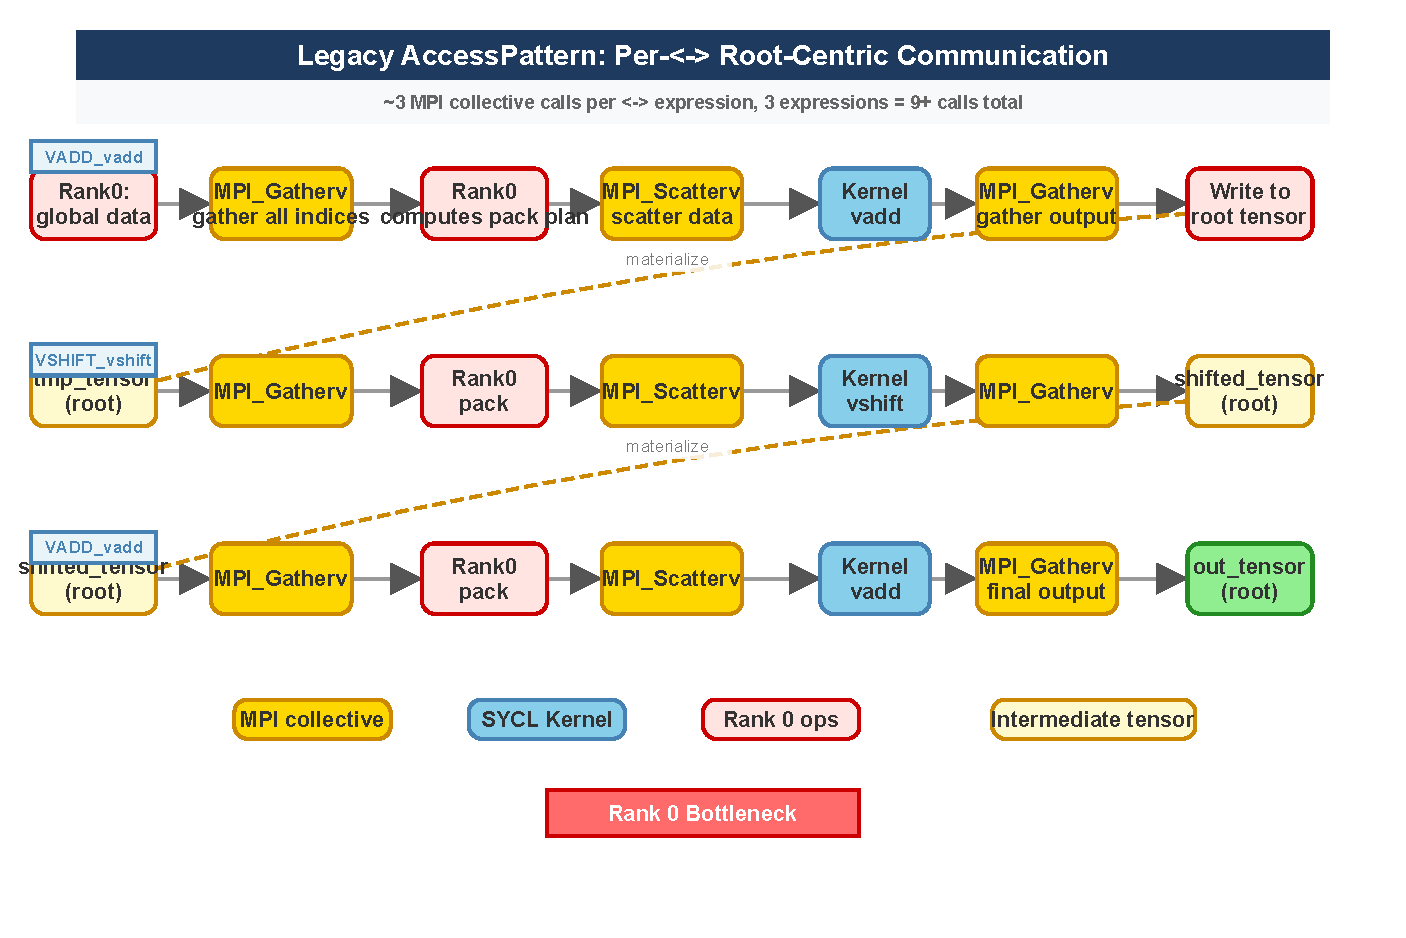
\includegraphics[width=0.85\textwidth]{figures/legacy_flow.pdf}
\end{figure}
\end{frame}

% ============ 第8页: 图2-Shell分区模型 ============
\begin{frame}{图示: Shell dataList → MPI Partition}
\begin{figure}
\centering
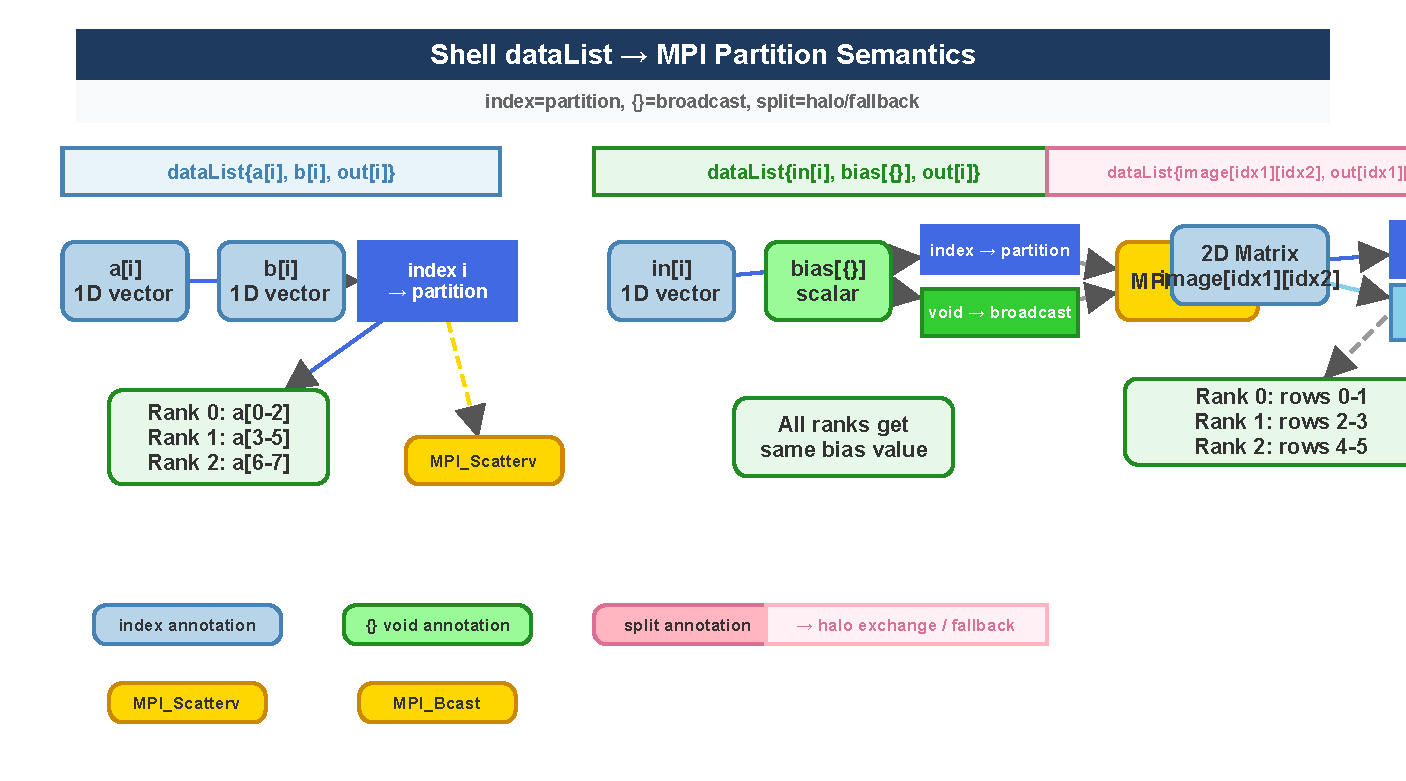
\includegraphics[width=0.85\textwidth]{figures/shell_partition_model.pdf}
\end{figure}
\end{frame}

% ============ 第9页: 图3-Operator Chain ============
\begin{frame}{图示: Operator Chain 中间张量驻留}
\begin{figure}
\centering
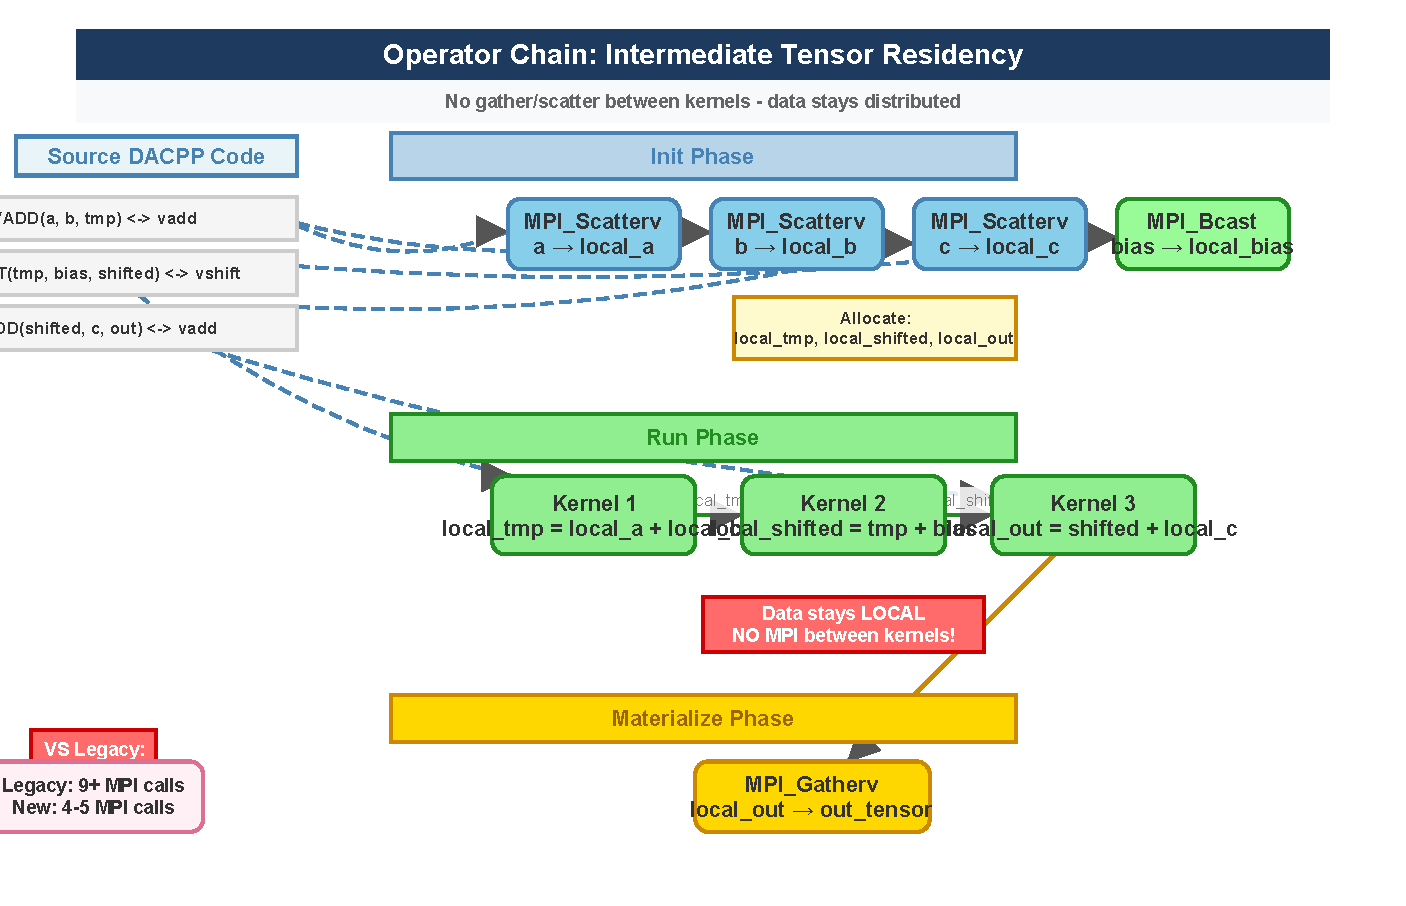
\includegraphics[width=0.85\textwidth]{figures/operator_chain.pdf}
\end{figure}
\end{frame}

% ============ 第10页: 通信次数对比 ============
\begin{frame}{通信次数对比}
\begin{block}{vectorAddCombo 示例}
\begin{center}
\begin{tabular}{lcc}
    \toprule
    方案 & MPI 调用次数 & 中间张量处理 \\
    \midrule
    Legacy AccessPattern & 9+ 次 & 每次 <-> 都 Gather/Scatter \\
    \textbf{新模型} & \textbf{4-5 次} & \textbf{仅 Init + Materialize} \\
    \bottomrule
\end{tabular}
\end{center}
\end{block}

\bigskip
\begin{columns}
\begin{column}{0.5\textwidth}
\begin{block}{Init Phase}
\begin{itemize}
    \item MPI\_Scatterv: a, b, c → local
    \item MPI\_Bcast: bias
    \item 分配 local buffers
\end{itemize}
\end{block}
\end{column}
\begin{column}{0.5\textwidth}
\begin{block}{Run Phase}
\begin{itemize}
    \item Kernel 1: local\_tmp = ...
    \item Kernel 2: local\_shifted = ...
    \item Kernel 3: local\_out = ...
    \item \textbf{无 MPI 调用!}
\end{itemize}
\end{block}
\end{column}
\end{columns}
\end{frame}

% ============ 第11页: 实现架构 ============
\begin{frame}{图示: 实现架构}
\begin{figure}
\centering
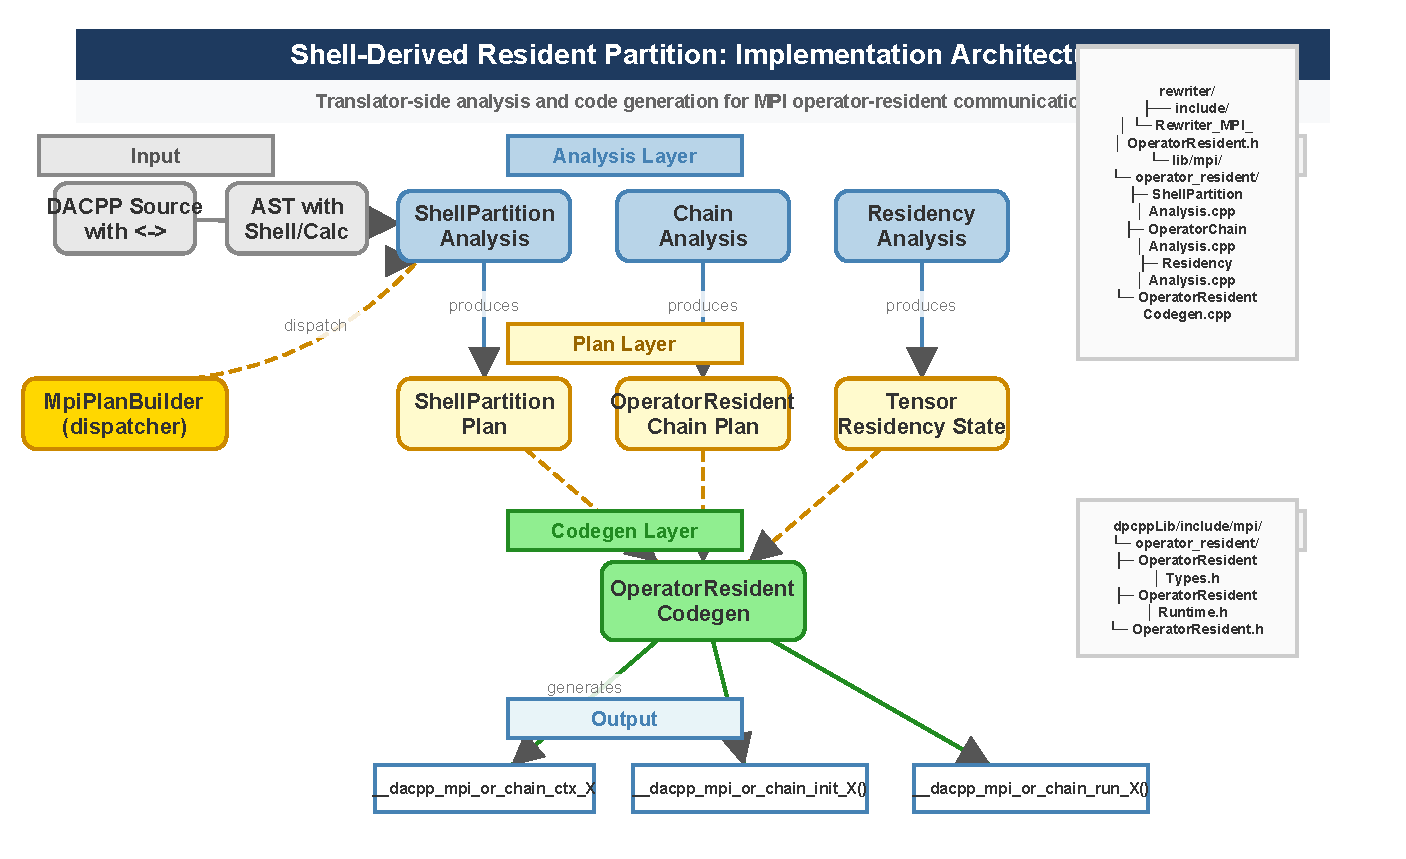
\includegraphics[width=0.9\textwidth]{figures/implementation_arch.pdf}
\end{figure}
\end{frame}

% ============ 第12页: 关键数据结构 ============
\begin{frame}{关键数据结构}
\begin{block}{ShellPartitionPlan}
\begin{itemize}
    \item bool supported
    \item std::string rejectReason
    \item std::vector<BindDomain> bindDomains
    \item std::vector<TensorDimMapping> mappings
    \item PartitionSignature signature
    \item std::vector<ParamAccessPlan> params
\end{itemize}
\end{block}

\bigskip
\begin{block}{PartitionSignature}
\begin{itemize}
    \item std::vector<int64\_t> bindSizes
    \item std::vector<int> bindOrder
    \item LocalLayoutKind layout
    \item std::string linearization
\end{itemize}
\end{block}
\end{frame}

% ============ 第13页: 实施阶段 ============
\begin{frame}{实施阶段}
\begin{block}{Phase 0: 结构探针}
\begin{itemize}
    \item 新增分析文件和头文件
    \item 对每个 <-> 打印 partition 分析结果
    \item 所有表达式仍走 legacy/stencil
\end{itemize}
\end{block}

\begin{block}{Phase 1: 1D direct mapped chain}
\begin{itemize}
    \item 接管 vectorAddCombo
    \item 支持 dataList\{a[i], b[i], out[i]\}
    \item 支持 bias[\{\}] scalar broadcast
\end{itemize}
\end{block}

\begin{block}{Phase 2: 2D row-block direct mapped}
\begin{itemize}
    \item 接管 imageAdjustment1.0
    \item 两个连续 image pass 共享 row ownership
\end{itemize}
\end{block}
\end{frame}

% ============ 第14页: Fallback 条件 ============
\begin{frame}{Fallback 条件}
\begin{block}{必须回退到 Legacy AccessPattern 的情况}
\begin{enumerate}
    \item \textbf{包含 RegularSplit}: 出现 split 标注 → stencil/halo 场景
    \item \textbf{Bind offset 非 0}: 第一版只接受 offset="0"
    \item \textbf{复杂 index 表达式}: 非简单仿射索引
    \item \textbf{链中间 host 读取}: 中间 tensor 被 print/tensor2Array 读取
    \item \textbf{READ\_WRITE 复杂别名}: 同一 tensor 有多个不兼容 writer
    \item \textbf{Partition 不兼容}: 连续 <-> 的 PartitionSignature 不一致
\end{enumerate}
\end{block}

\bigskip
\begin{alertblock}{设计约束}
\begin{itemize}
    \item 不改源码语法 (<-> 不变)
    \item 不改 CLI 参数
    \item 不改运行时 include 路径
    \item 不影响 stencil Phase-C 主路径
\end{itemize}
\end{alertblock}
\end{frame}

% ============ 第15页: 总结 ============
\section{总结}
\begin{frame}{总结}
\begin{block}{核心改进}
\begin{enumerate}
    \item \textbf{通信主轴转变}: 从 "每个 <-> 每个参数访问哪些 index" → "dataList 如何定义迭代域和划分"
    \item \textbf{中间张量驻留}: 链内中间 WRITE 不 Gather/Scatter
    \item \textbf{消除间接寻址}: 连续可直访时使用 ContiguousView
    \item \textbf{统一 fallback}: 不支持的模式回退 legacy，不改变语义
\end{enumerate}
\end{block}

\bigskip
\begin{block}{预期收益}
\begin{itemize}
    \item vectorAddCombo: 9+ → 4-5 次 MPI 调用
    \item imageAdjustment1.0: 避免中间 image tensor 往返
    \item 通信结构接近手写 MPI+SYCL 参考实现
\end{itemize}
\end{block}
\end{frame}

% ============ 第16页: 谢谢 ============
\begin{frame}
\begin{center}
\Large Thank You! \\
\bigskip
\large Questions?
\end{center}
\end{frame}

\end{document}
